%\documentclass[12pt,preprint]{aastex}
%\documentclass[preprint2,12pt]{aastex}
\documentclass{emulateapj}
%\usepackage{apjfonts}
\usepackage{graphicx}
\usepackage{amssymb}
\usepackage{amsmath}

\shortauthors{Name et al.}
\shorttitle{Best transiting planets}

\begin{document}

% ------------------------------------------------------------------------
% New commands
%
\def\ltsima{$\; \buildrel < \over \sim \;$}
\def\lsim{\lower.5ex\hbox{\ltsima}}
\def\gtsima{$\; \buildrel > \over \sim \;$}
\def\gsim{\lower.5ex\hbox{\gtsima}}
\def\tess{{\it TESS} }
\def \teff {T_{\rm eff}}
\def \phir {\Phi_{\rm R}}
\def \fov {24$^{\circ}$}
\def \pixsz {21.1''}
\def \aeff {69.1 cm$^2$ }    
\def \epd {105 mm}                          
                                                                                          
% -------------------------------------------------------------------------
%

\bibliographystyle{apj}

\title{ A Toy Analytic Transit Survey: Fixed Light Ratio Binaries }

\author{
  LGB, KM, JNW
}

% \journalinfo{Draft version}
\slugcomment{Memo for internal use}

%\altaffiltext{1}{Princeton University}

\begin{abstract}

We discuss various errors one can make by ignoring binarity when deriving 
occurrence rates.
In this memo, we assume the stars in any binary system have fixed light ratio.

\end{abstract}

\keywords{planets and satellites:\ detection}

\section*{Statement of problem}

Ah, transiting planets! We learn so much by studying them. But how much can we 
actually learn, and how much is messed up by binarity?

Imagine the following survey, similar to that outlined by [Pepper et al, 2003]:
\begin{enumerate}
\item You are going to observe the entire sky for a duration $T_{\rm obs}$, 
with a detector of area $A$, and known bandpass. Your detector is photon-noise 
limited.
%
\item You are interested only in detecting planets of radius $R_p$, and orbital 
period $P$. For instance, $R_p=R_\oplus$, $P={\rm 1\ year}$.
%
\item You only want to detect them around stars of radius $R_1$, and luminosity 
$L_1$. For instance, G2V dwarfs.
%
\item Since your detections will be S/N limited, you want only to observe stars 
for which your target can be detected with ${\rm S/N} > {\rm (S/N)_{min}}$.
%
\item For a photon-noise limited survey, the signal to noise limit is 
equivalent to a magnitude (flux) limit. So you select all the points on the sky 
above a flux limit, \textit{i.e.} with flux $F_{\rm pt} > F_{\rm min}$, for 
$F_{\rm min}$ defined by your target planet and stellar types, and your survey 
specifications.
%
\item You carry out a transit survey, and detect many transiting planets.
\end{enumerate}

You now wish to derive an occurrence rate for planets of radius $R_p$ and 
orbital period $P$.
Assume your universe is a universe in which:
\begin{itemize}
\item The true population of ``points'' (stellar systems, all unresolved) 
	comprises both single and double star systems. Single star systems have 
	luminosity in the observed bandpass $L_1$, radii $R_1$, and effective 
	temperature $T_{\rm eff,1}$.
	Double star systems have luminosity in the observed bandpass $L_d = 
	(1+\gamma_R)L_1$, for $\gamma_R = L_2/L_1$ the ratio of the luminosity of 
	the secondary to the primary. 
  In this memo, $\gamma_R$ is assumed to be a constant across the population of
  star systems.
  The ratio of the two number densities in a 
	volume-limited sample is the binary fraction\footnote{The binary fraction 
	is equivalent to the multiplicity fraction if there are no triple, 
	quadruple, $\ldots$ systems.}.
\item The true population of planets around these stars is as follows:
	\subitem A fraction $\Gamma_{t,s}$ of stars in single star systems 
	have a planet of radius $R_p$, with orbital period $P$.
	\subitem A fraction $\Gamma_{t,d}$ of each star in a double star 
	system has a planet of radius $R_p$, with orbital period $P$. For instance, 
	if $\Gamma_{t,s} = \Gamma_{t,d} = 0.1$, on average each double 
	system contributes 0.2 planets, and each single system 0.1 planets.
    Any astrophysical difference in planet formation between singles and 
    binaries is captured by these two terms.\footnote{We'll see that it's 
    an extreme limit to assume the primary and secondary of binary systems host 
    planets at equal rates if the secondary is non-identical to the primary.}
\end{itemize}


Consider the following set of questions:
\begin{enumerate}
\item How many single and double star systems, respectively, are in the sample?
Correspondingly, how many stars are in the sample?

\item How many planets are in the sample? (Orbiting single stars, and orbiting 
double stars respectively).

\item What is the true occurrence rate?

\item How many planets are detected?

\item What occurrence rate does astronomer A, who has never heard of binary 
star systems, derive for planets of radius $R_p$ and period $P$?

\item What occurrence rate does astronomer B, who accounts for the ``2 for 1'' 
effect of binarity (\textit{i.e.} that the sample actually has more stars than 
astronomer A thought) derive?

\item What about astronomer C, who accounts for ``2 for 1'' \textit{and} 
misclassification due to diluted radii? In other words, astronomer C did a 
combination of high resolution imaging and RV followup on every candidate, and
correctly classifies the planetary radii in every case.
\end{enumerate}


\section{How many stars are in the sample?}

Let $N_s$ be the number of single star systems, and $N_d$ the number of double 
star systems. Then the total number of stars in the sample can be written
\begin{equation}
N_{\rm stars} = N_s + 2N_d.
\end{equation}

In a magnitude-limited sample in which stars are uniformly distributed in 
volume, the number of stars will be the number density times the volume.
If the volume is taken to be a sphere over which the number density is uniform,
\begin{equation}
N_i = n_{i} \frac{4\pi}{3} d_{{\rm max},i}^3,
\label{eq:number_systems}
\end{equation}
for $i\in{\rm \{single,double\} } \equiv { \{s,d\} }$, and
\begin{equation}
\frac{n_{d}}{n_{s}} = {\rm binary\ fraction} \equiv {\rm BF}
\end{equation}
by definition. The absolute normalization of the number density is a measured 
quantity, as is the binary fraction. For G2V dwarfs, the latter is $\approx 
0.45$ [Duchene \& Kraus, 2013]. The former is given by [Bovy 2017].

$d_{{\rm max},i}$ in Eq.~\ref{eq:number_systems} is the maximum distance 
corresponding to the given magnitude limit:
\begin{equation}
d_{{\rm max},i} = \left(\frac{L_{i}}{4 \pi F_{{\rm lim}}}\right)^{1/2},
\label{eq:d_max}
\end{equation}
where the limiting flux in the bandpass $F_{{\rm lim}}$ can also be 
stated in terms of the limiting magnitude $m_{{\rm lim}}$,
\begin{equation}
m_{{\rm lim}} = m_{0} - \frac{5}{2} \log_{10} \left(\frac{F_{{\rm 
lim}}}{F_{0}}\right),
\end{equation}
for $m_{0}$ a zero-point magnitude and $F_{0}$ its corresponding flux (as 
always, everything is implicitly written in a defined bandpass).

In Eq.~\ref{eq:d_max}, again $i\in{\rm \{single,double\} }$, and as a 
consequence the maximum distance to which binary stars will be selected is 
greater than that of single stars, simply as a consequence of imposing a 
magnitude cut.
The ratio of double to single systems, assuming $\gamma_R$ is a constant for 
the entire population, is
\begin{align}
\frac{N_d}{N_s} &= 
	\frac{n_d}{n_s} \left(\frac{d_{{\rm max}, d} }{d_{{\rm max}, s}}\right)^3 \\
&= {\rm BF} \times (1+\gamma_R)^{3/2}.
\end{align}
In the nominal case of twin binaries ($\gamma_R = 1$), with a binary fraction 
${\rm BF} = 0.5$, there are 
$\sqrt{2}$ more binary systems than single systems in the sample.
Correspondingly, there are $2\sqrt{2}$ more stars in binary systems than stars 
in single systems.

As a comment on Eq.~\ref{eq:number_systems}, if 
we wished to write a stellar number density profile that accounted for the 
vertical structure of the Milky Way, we might choose a profile either 
$\propto \exp(-z/H)$, or $\propto {\rm sech}^2(z/H)$ for $z$ the distance from 
the galactic midplane and $H$ a scale-height. Both density profiles would lead 
closed form analytic solutions.

\subsection{Actually finding $F_{\rm lim}$}

To express $F_{\rm lim}$ in terms of the survey's defining parameters, we need 
to convert between ${\rm (S/N)_{lim}}$ and $F_{\rm lim}$. We proceed as follows.

The signal ${\rm S}$ for a box-car train transiting planet is
\begin{align}
{\rm S} &= \delta \mathcal{D} \\
&= \left(\frac{R_p}{R_\star}\right)^2 \mathcal{D},
\end{align}
for $R_p$ the planet's radius, $R_\star$ that of its host star, and 
$\mathcal{D}$ the dilution parameter defined as
\begin{equation}
\mathcal{D} = 
\Bigg\{\begin{array}{lr}
L_1 / L_d, & {\rm\ if\ binary\ and\ target\ primary}\\
\gamma_R L_1 / L_d, & {\rm\ if\ binary\ and\ target\ 
	secondary}\\
1, & {\rm\ if\ single},
\end{array}
\label{eq:dilution}
\end{equation}
where $L_1, L_d,$ and $\gamma_R$ were defined in the opening monograph.

Assuming the only source of noise is Poissonian counting noise, the noise ${\rm 
	N}$ can be written
\begin{equation}
{\rm N} = \frac{1}{\sqrt{N_\gamma}},
\end{equation}
for $N_\gamma$ the number of photons received by the detector. This noise model 
is a useful simplification -- see [Howell 2006, pg 75] for the full 
CCD equation.
The number of received photons can be written
\begin{equation}
N_\gamma = F^{\rm N}_\gamma A N_{\rm tra} T_{\rm dur},
\end{equation}
for $F^{\rm N}_\gamma$ the photon number flux from the system [${\rm 
	ph\,cm^{-2}\,s^{-1}}$], 
$A$ the detector area, $T_{\rm dur}$ the transit duration, and $N_{\rm tra} $ 
the number of transits observed, which is multiplied in assuming the transits 
are ``phase-folded''.

Thus the signal to noise ratio can be written
\begin{equation}
{\rm S/N} = \delta \mathcal{D} \sqrt{F^{\rm N}_\gamma A N_{\rm tra} T_{\rm 
		dur}}.
\label{eq:snr_ivory_tower}
\end{equation}

In passing, given the parameters that define a survey and planet type, 
Eq.~\ref{eq:snr_ivory_tower} would need to be re-expressed with 
$N_{\rm tra}$ roughly the ratio of the observing baseline to the planet period, 
and $T_{\rm dur}$ a function of $R_\star, P, a$, and impact parameter $b$, and 
then perhaps averaged over $b$. We leave them as-is for subsequent 
development.

Using Eq.~\ref{eq:snr_ivory_tower}, we can write the minimum number flux of 
photons required for a detection at threshold as
\begin{equation}
F_{\rm lim}^N = \left[ \left({\rm \frac{S}{N}}\right)_{\rm min} \frac{1}{\delta 
\mathcal{D}} \right]^2 \frac{1}{A N_{\rm tra} T_{\rm dur}}.
\end{equation}
To convert this to $F_{\rm lim}$, multiply by the average photon energy in the 
bandpass.



\section{How many planets are in the sample?}

The number of planets in the sample is
\begin{align}
N_{\rm planets} =& N_{\rm planets\ in\ single\ star\ systems}  +  \\
				  &\quad\quad N_{\rm planets\ in\ double\ star\ systems} 
				  \nonumber \\
			   =& \Gamma_{t,s} N_s + 2 \Gamma_{t,d} N_d.
\end{align}

The factor of 2 accounts for the fact that there are twice as many stars in 
double star systems.



\section{What is the true occurrence rate?}
\label{sec:true_rate}

The ``true occurrence rate'' is the average number of planets per star. Thus

\begin{align}
\Gamma_t &= \frac{N_{\rm planets}}{N_{\rm stars}} \\
\Gamma_t &= \frac{\Gamma_{t,s} N_s + 2 \Gamma_{t,d} N_d}{N_s + 2N_d}.
\label{eq:true_occ}
\end{align}



\section{How many planets are detected?}
The total number of planet detections is the sum of the number of planets 
detected in single star systems $N_{{\rm det},s}$ and the number of planets 
detected in double star systems $N_{{\rm det},d}$.
These can be expressed individually. 
Since we selected stars for which there was enough light to make detections, 
there is no need to compute the ${\rm S/N}$ distribution of 
``threshold-crossing events''.

The number of planets detected in single star systems is
\begin{equation}
N_{{\rm det},s} = N_s \Gamma_{t,s} f_{s,{\rm geom}},
\label{eq:N_det_s}
\end{equation}
where the product $N_s \Gamma_{t,s}$ is the number of planets in the single 
star systems of the sample, and $f_{s,{\rm geom}}$ is the geometric transit 
probability.
The number of planets detected in double star systems is
\begin{equation}
N_{{\rm det},d} = 2 N_d \Gamma_{t,d} f_{d,{\rm geom}},
\label{eq:N_det_d}
\end{equation}
where now $2 N_d \Gamma_{t,d}$ is the number of planets in the double star 
systems of the sample.
The number of detected planets $N_{\rm det}$ is the sum of the two previously 
written equations.


\section{Astronomer A ignores binarity}
Astronomer A has never heard of binary star systems. What occurrence rate does 
he derive for planets of radius $R_p$ and period $P$?

The {\it total} occurrence rate (number of planets divided number of 
``stars'') for Astronomer A would be $(N_{\rm det}/f_{s,{\rm geom}})/(N_s + 
N_d)$. However, even though Astronomer A does not know about binaries, the 
radii he derives for any planets in binary systems are too small, by a factor 
$\sqrt{\mathcal{D}}$. The question asks what occurrence rate is derived for 
planets of radius $R_p$ and period $P$.
The answer is
\begin{align}
\Gamma_{\rm A,\ planets\ of\ R_p} &= \frac{N_{\rm det,s}/f_{s,{\rm geom}}}{N_s 
+ N_d}
\label{eq:A_0} \\
&= \frac{\Gamma_{t,s} N_s}{N_s + N_d}
\end{align}

This astronomer will also think there is a second population of planets, with 
radius $R_p \sqrt{\mathcal{D}}$ (a constant number for $\gamma_R = {\rm 
constant}$). He will then also claim
have derived a second occurrence rate,
\begin{equation}
\Gamma_{\rm A,\ planets\ of\ R_p \sqrt{\mathcal{D}}} = \frac{N_{\rm 
det,d}/f_{d,{\rm geom}}}{N_s + N_d},
\end{equation}

where at least for the twin binary case the geometric completeness term is the 
same as for Eq.~\ref{eq:A_0}.


\section{Astronomer B counts host stars correctly}
Astronomer B can somehow account correctly for the ``2 for 1'' 
effect of binarity, \textit{i.e.} that the sample actually has more stars than 
astronomer A thought.

By the same token as above,
\begin{equation}
\Gamma_{\rm B,\ planets\ of\ R_p} = \frac{N_{\rm det,s}/f_{s,{\rm geom}}}{N_s + 
2N_d},
\end{equation}
and
\begin{equation}
\Gamma_{\rm B,\ planets\ of\ R_p \sqrt{\mathcal{D}}} = \frac{N_{\rm 
det,d}/f_{d,{\rm geom}}}{N_s 
	+ 2N_d}.
\end{equation}



\section{Astronomer C counts host stars correctly and figures out diluted radii}
Astronomer C did high resolution imaging followup on every candidate, and 
correctly classifies the planetary radii.
Thus, she also knows which planets are in binary systems, and which are in 
single star systems.
Since there are no completeness corrections, she has everything she needs.

She knows that the purported population of planets with radii $R_p 
\sqrt{\mathcal{D}}$ does not exist. All detected planets from this survey have 
radii $R_p$. She computes an occurrence rate
\begin{align}
\Gamma_{\rm C,\ planets\ of\ R_p} &= 
\frac{N_{\rm det,s}/f_{s,{\rm geom}} + N_{\rm det,d}/f_{d,{\rm geom}}}{N_s + 
2N_d} \\
&= \frac{\Gamma_{t,s} N_s + 2\Gamma_{t,d} N_d}{N_s + 2 N_d}.
\end{align}

With $\approx$ a full semester at Keck, a system-by-system analysis, 
and perfect understanding of the completeness of the detection efficiency for 
single and double star systems, Astronomer C has found the true occurrence rate 
(cf. Eq.~\ref{eq:true_occ}).




\section{Numerical verification}

As a check on the preceding analytic discussion, we implemented a Monte Carlo 
simulation of this idealized transit survey.
To run the survey, we defined the instrument specifications (detector area and 
transmission function), the stellar population (binary fraction, total number 
density of a given stellar class, binary light ratio, fixed stellar 
properties), the planet population (fixed planet radius, period, and occurrence 
rate about single and binary stars), and finally the survey parameters 
(observing baseline, minimum SNR for ``detection'').
We then randomly drew star positions, randomly assigned planets to stars in 
single and binary systems, and computed the resulting signal to noise 
(Eq.~\ref{eq:snr_ivory_tower}) with which 
the transits would be observed.
As in the preceding analytics, we assumed ``twin'' binaries (same stellar 
radii, same effective temperature, and dilution does not depend on which 
stellar binary is the ``target'').

The results are shown in Fig.~\ref{fig:snr_dist_analytic_v_numeric}, and 
indicate that the analytic probability distribution functions derived in an 
earlier version of this memo are correct.

A point evident in Fig.~\ref{fig:snr_dist_analytic_v_numeric} is that, for 
fixed planet parameters, and fixed stellar parameters ($R_\star, L_\star$, and 
distance $r$), and a constant $\gamma_R$ across the population, the SNR 
distribution for planets in binaries is poorer than that of planets in single 
star systems.
We can see analytically that this can be written only as function of the 
binary light ratio:
\begin{equation}
\frac{{\rm prob}(x_d)}{{\rm prob}(x_s)} =(1 + \gamma_R)^{-1}.
\end{equation}
Deriving this simple form requires noting that the ratios of the 
bandpass-specific number luminosities is equal to the ratio 
of the bandpass-specific energy luminosities (otherwise a term with $c_s/c_d$ 
must be included).

\begin{figure}[!t]
	\begin{center}
		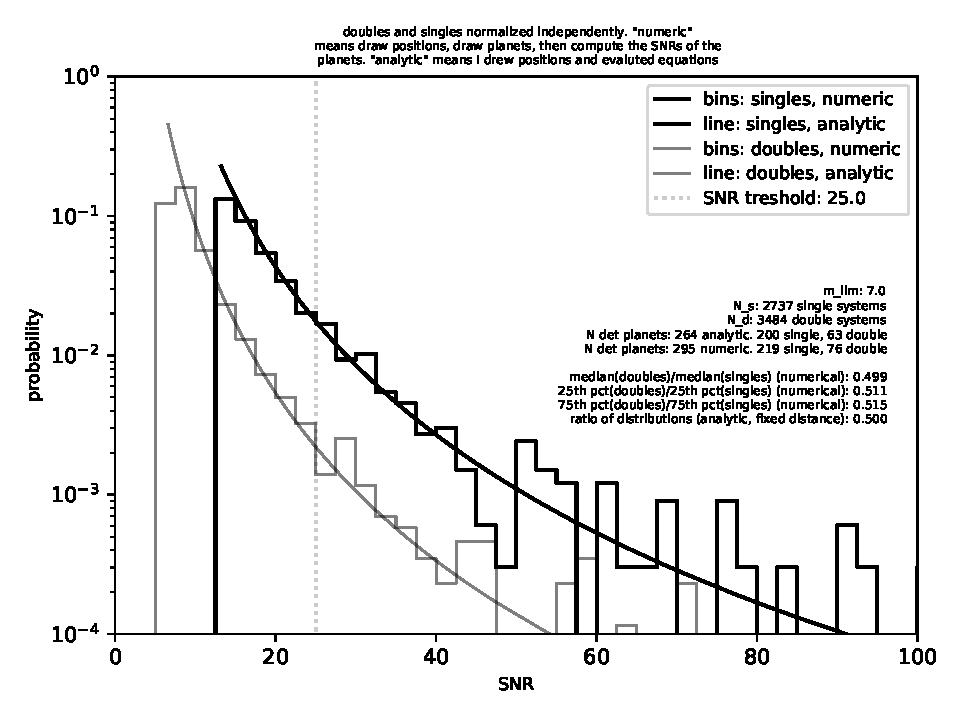
\includegraphics[scale=0.4]{figures/snr_distribution.pdf}
	\end{center}
	\caption{Comparison of analytic and numeric probability 
	density functions of the SNR in an idealized transit survey.
	The analytic lines are from a previous version of this memo 
	(\texttt{20170728}) for the planet populations orbiting single and binary 
	stars. The underlying stepped histogram is output from Monte Carlo 
	simulations. Poisson noise leads to a small deviation at the faint and 
	bright limits, but the numerics and analytics otherwise agree.
		 }
	\label{fig:snr_dist_analytic_v_numeric}
\end{figure}


\section{Representative numbers for a few cases}

\subsection{Twin binaries: if we ignore binarity, for what fraction of 
detections do we misclassify the radii?}
 
Ignoring binarity, we will detect $N_{\rm det,s}$ planets around single stars, 
and $N_{\rm det,d}$ planets around double stars. The latter set will be assumed 
to have radii $R_p \sqrt{\mathcal{D}}$.
The fraction of detections with misclassified radii can then be written
\begin{equation}
\frac{N_{\rm det,d}}{N_{\rm det,s} + N_{\rm det,d}} = \frac{1}{1+\alpha},
\end{equation}
for
\begin{equation}
\alpha \equiv \frac{1}{2({\rm BF})} (1+\gamma_R)^{3/2} 
\frac{\Gamma_{t,s}}{\Gamma_{t,d}}.
\end{equation}

For the nominal G2V dwarf case of ${\rm BF}=0.45$, twin binaries with equal 
occurrence rates this produces a misclassification rate of $24\%$, in agreement 
with Fig.~\ref{fig:snr_dist_analytic_v_numeric}.

\subsection{Twin binaries: if we ignore binarity, how wrong is our occurrence 
rate for planets of radius $R_p$?}

This is almost simply asking ``what is the relative difference between the 
occurrence rates derived by Astronomers D and A for planets of radius $R_p$?''
However, in the more realistic case, Astronomer A also has derived a 
completeness, which we assume is the same as for Astronomer D in the single 
star case.
So Astronomer A now misclassifies planetary radii, and miscounts the total 
number of stars, but knows his completeness for single stars.
Astronomer D corrects all these errors.

For brevity, write $\Gamma_{\rm A,\ planets\ of\ R_p} = \Gamma_{\rm A,R_p}$, 
and similarly for ${\rm D}$.
Then the relative difference between the two occurrence rates is

\begin{align}
\left|\frac{\Gamma_{\rm A,R_p} - \Gamma_{\rm D,R_p}}
		   {\Gamma_{\rm A,R_p}} \right| &=
\left| 1 - \frac{\Gamma_{\rm D,R_p}}{\Gamma_{\rm A,R_p}}\right| \\
&=
\left| 1 - \left(\frac{\Gamma_{t,s}N_s + 2\Gamma_{t,d}N_d}{N_s + 2N_d}  \cdot 
\frac{N_s + N_d}{\Gamma_{t,s} N_s }\right)\right| \\
&= 
\left|
1 - \frac{(1 + 2 \beta \Gamma_{t,d}/\Gamma_{t,s})(1 + \beta)}{(1+2\beta)}
\right|,
\end{align}
for
\begin{equation}
\beta \equiv N_d/N_s = {\rm BF} \times (1+\gamma_R)^{3/2}.
\end{equation}

For the nominal G2V dwarf case of ${\rm BF}=0.45$ with twin binaries ($\gamma_R 
= 1$) and $\Gamma_{t,d} = \Gamma_{t,s}$ this gives a relative error of $127\%$.
For instance, in the numerical simulation corresponding to 
Fig.~\ref{fig:snr_dist_analytic_v_numeric}, Astronomer A finds $\Gamma_{\rm 
A,R_p} = 0.22$, while Astronomer 
D derives the true (input) occurrence rate of $\Gamma_{\rm D,R_p} = 0.5$.
For the more ``realistic'' case of $\gamma_R = 0.1$, $\Gamma_{t,d} = 
\Gamma_{t,s}$, the relative error is $52\%$. Not as bad, and this latter number 
should be looked at skeptically because the ``equal occurrence rates for 
primary and secondary'' assumption may be unlikely with this light ratio as a 
median.

\newpage



%\begin{thebibliography}{}


%\end{thebibliography}

\end{document}
